\chapter{Background}
\label{cha:background}

In this chapter we aim to provide the reader with a concrete understanding of key concepts utilised within our new tomographic technique along with a conceptual grasp on metrics and methods used to analyse and verify it. We begin with the theory and intuition behind previously and currently employed random network generation algorithms in \cref{sec:Bgraphgeneration}, providing the reader with a deeper understanding of terms from \cref{ssec:Icurrentmodels}.\par
To explore findings within previous work relating to the effect of monitor placements strategy on tomographic accuracy, we introduce established algorithms for placement of these observable monitors within networks from literature in \cref{sec:Bmonitorplacement}. Next we establish the requirement for discriminatory probe path routing within the network and draw real world analogues for hypothetical routing constraints, we also separate routing into four classes according to these restraints, justifying a focus on the \cbr and \cfr mechanisms for subsequent sections.\par
Next we give generalised explanations of key statistical concepts, concisely summarizing their realization within our work in \cref{sec:Bparameterestimation} and \cref{sec:Boptimization} with the intent of giving a more verbose grounding of these in the context of network tomography within \cref{cha:methodology}. Lastly we tie all aforementioned concepts together through their use within our novel tomographic model and explore existing implementations of \pdv tomography within the network tomographic corpus in \cref{sec:Maddtomography}.

\section{Graph Generation}
\label{sec:Bgraphgeneration}

Monitors in the case of this model function as normal switches with regards to packet generation and reception but perform additional recording functionality. Each monitor stores information pertaining to each packet which is generated or received by itself. This stored information is analogous to a traceroute of the packet's path through the network; a list of routers that the packet has passed through. The monitors also store the total time taken by the packet for it’s traversal, as well as the source and destination IP.\par
Within the graph resulting from the network generation, all edges are undirected and represent links between machines (router, switches or monitors). For simplicity each distinct pair of nodes may only be linked by a single edge, however multiple physical links between a pair of machines occur in the real world, the edge can be considered a virtual aggregation of all of these links, representing their total cumulative throughput. Each node within the graph is a representation of a physical piece of networking hardware, either a router or switch, these are simplified abstractions of their real world analogous, with their key simplifications being those enumerated in the previous section.\par
The current network generation strategy follows that of the Erdős–Rényi (ER) model; this was introduced by \cite{gilbert_random_1961} and later that year revisited in “On Random Graphs I.” by the model’s titular author pair \cite{erdos_random_1959}. This random graph generation is characterised by each node in a graph being connected to each other node with a predefined probability of $p$, that is for a graph \gls{network} with $n>1$ nodes and a connectivity probability $0\leq p\leq 1$, $G=f(n,p)$.\par
This random graph generation strategy is intuitive in its simplicity however has several problems when used to generate graphs analogous to computer networks. The most prominent shortcomings are in the node degree distribution and presence of so called ‘isolated nodes’. A key underlying assumption of the ER model is that each edge between two nodes is equally likely to occur within a graph. The natural consequence of this assumption is that the distribution of node degree’s (number of connected edges) within the graph approximates a Poisson distribution (\cite{albert-laszlo_scale-free_2003}). Such random networks are referred to as exponential networks as the probability that a node is connected to $n$ other nodes decreases exponentially as $n\to\infty$.\par
Complex networks however have not been observed to follow a random pattern but rather that, irrelevant of age, function or scope converge to a similar architecture as shown in \cite{albert_diameter_1999}’s mapping of the world wide web . This network architecture has been dubbed as scale-free and is characterised by the distribution of node degree following a power-law where the probability of a node having $k$ edges $P(k)$  is proportional to $\frac{1}{kn}$ for a network of $n$ nodes. This property is present in graphs generated using the Barabási–Albert (BA) model, as well as the Watts–Strogatz model; these generation techniques among others are further discussed in \cref{cha:background}.\par
As the network being generated and analyzed continues to increase in size we expect its behaviour and structure to become increasingly complex. Given this complex nature the scale-free property of graph generation is highly desirable for generation of pseudo realistic networks.

\section{Monitor Placement}
\label{sec:Bmonitorplacement}
Within \gls{network} there is a set of switches \gls{switches} analogous to connections with external networks, such as the internet as outline in \cref{cha:intro}. Within this set of switches we distinguish a set of monitors $\gls{monitors}\subseteq \gls{switches}$ which we are able to directly observe and control. In all forms of tomography use observations obtained from $M$ to infer the state of \gls{network}, as such the selection of \gls{monitors} has a substantial impact on the inference we are able to obtain regarding \gls{network}. Previous work has explored placement strategies of \gls{monitors} given the topology of \gls{network}, we focus on the three algorithms derived from these strategies in \cite{ma_optimal_2015}:
\begin{enumerate}
    \item Random placement algorithm
    \item Greedy placement algorithm
    \item Ma's algorithm
\end{enumerate}

\todo{Show monitor placement examples in a set topology (7 router like Barnes)}

\section{Routing Mechanisms}
\label{sec:Broutingmechanisms}

    In this work we use the term probe packets to denote UDP packets sent between monitors which differ from other traffic by their transfer from and to uniquely identifiable ports on the sending and receiving switch. Probe packets are allocated on a per packet basis to a unique path through the network (referred to as a probe path) which is a directed path through a series of routers which the packet is guaranteed to take by the routing protocols unless it is dropped due to a router buffer within the path being full. Each probe path in the set of selected probe paths (denoted as $P$) is uniquely identified by the monitors it is between and the set of routers it traverses. The probe path a packet is taking is noted though the packet's respective transmission/reception port and additional explicit notation within the data section of the packet, we further elaborate on the technical representation of these probe paths in \cref{sec:Mnetworkprobing}.\par
    
    Given we assume a priori knowledge of the network's topology a set of probe paths is decided on before beginning to collect end-to-end measurements. At the beginning of the measurement interval each monitor sends an allocated number of probe packets along each probe path, noting the time sent ($t^s$) and along which probe path. The destination monitor upon reception of the packet then also stores the time of reception ($t^r$) and packet's probe path, as illustrated in \ref{fig:pptransmission}. 
    \begin{figure}[H]
        \centering
        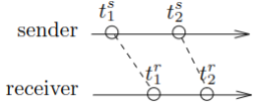
\includegraphics[width=5cm]{figs/background/probe_transmission.png}
        \caption[Illustration of probe packet transmission between two monitors]{Illustration of probe packet transmission between two monitors \protect\cite{he_fisher_2015}}
        \label{fig:pptransmission}
    \end{figure}\newpage
    \noindent Given $n$ probes are sent on a path we are then able to find the mean end-to-end travel time of a packet on that path by: \[\text{travel time}=\frac{\sum_{i=1}^nt_i^r - t_i^s}{n}\] where $t_n^s$, $t_n^r$ denote the time the $x$th packet sent on that path is sent and received respectively. This calculation is trivial within small networks as there exist only a small number of probe paths and the measurement interval (and therefore $n$) required for reliable metrics is brief. To account for clock synchronization discrepancies between distributed monitors in this calculation we introduce the concept of packet delay variation (PDV) tomography for analysis in \cref{sec:Mnetworkprobing} \par

    Let \gls{monitors} denote the set of monitors within \gls{network}, \gls{ppaths} denote the set of all possible probe paths, and $\gls{|}P|$ be the number of potential probe paths  is then intuitively equal to all possible non cyclic paths between each pair of monitors. A naive approach of calculating all probe paths is therefore of the order $\mathcal{O}(m^m)$ where $m=\gls{|}\gls{monitors}|$. As the network grows in size this super-exponential growth of possible probe paths requires a more discerning approach to probe path selection. As the ultimate goal of our end-to-end probing is to enable identifiability of each router within the network we need only ensure the chosen set of probe paths is sufficient for this identification.\par
    
    Unique router identification via probing is dependant on the flexibility afforded by the probe packet routing mechanism, we employ terminology from \cite{he_network_2021} and split these routing mechanisms into 4 groups: \begin{itemize}
        \item Uncontrollable routing (UR)
        \item Controllable cycle-free routing (CFR)
        \item Controllable cycle-based routing (CBR)
        \item Arbitrarily controllable routing (ACR)
    \end{itemize}As these mechanisms dictate $P$ they define the identifiability of each router given $M$ or inversely the bounds of $|M|$ and what position within the network each $m\in M$ must be to uniquely identify each router.\par
    Uncontrollable routing refers to when P is limited to only paths that the background traffic's link-state routing protocol establishes, given the dynamic nature of this routing we are unable to established a fixed $P$ violating the assumptions of our probe path routing, as such we will not consider UR in our analysis. Previous work in \cite{barnes_stochastic_2020} has established that in a stochastic routing network using UR for probe paths router identifiability cannot be established and a prohibitively computationally expensive Markov Chain Monte Carlo (MCMC) (\cite{dellaportas_bayesian_2002}) based estimation method must be used instead.\par
    
    Arbitrarily controllable routing represents the ideal case where a probe packet traverse every link and router as many times as desired. This form of routing is analogous to that afforded by SDN and other strict source routing architectures (\cite{university_of_southern_california_darpa_1981}, \cite{open_networking_foundation_openflow_2015}) and allows for complete router identifiability using only a single arbitrarily placed monitor (\cite{he_network_2021}). Due to the triviality of router identification and limited SDN use cases in real world networks (\cite{jarschel_interfaces_2014}) under this scheme we will not consider ACR in our analysis.\par
    
    The remaining routing mechanisms CBR and CFR represent routing mechanisms within all optical (\cite{ahuja_srlg_2011}) and multi protocol label switching (MPLS) networks (\cite{rosen_multiprotocol_2001}) respectively. In CBR a packet may traverse a router any number of times but only traverse each link once, in contrast under CFR a packet may only traverse every router and link at most once. As routing restrictions under CBR are relaxed compared to those under CFR we note that for all topologies $max(P)|CFR \subseteq max(P)|CBR$. Both these mechanisms are widely used and provide an interesting set of limitations while still allowing for unique router identifiable, we will therefore focus on these in our analysis, mentioning UR and ACR only in relevant edge cases.

\section{Parameter Estimation}
\label{sec:Bparameterestimation}

In this section we define and explain the fundamental statistical concepts underpinning the optimisation methods for our tomographic analysis. We note that a network as we have defined it is composed of only nodes (routers, switch and monitors) and physical uniform links, inferences made about a network are analogous to inferences of nodes and links. These concepts extend on statistical methods in the context of network science form \cite{meng_method_2016}, \cite{he_fisher_2015}, and \cite{he_network_2021}, re-framing them for application in the context of tomographic identification of nefarious routers.\par
The first of these key concepts is Maximum Likelihood Estimation (MLE) to determine the node and link level parameters which give the highest chance of having observed the given packet delays and losses at monitor nodes. The second is the notion of Fisher Information to quantify both the amount of knowledge we have about the underlying network and the accuracy of our MLE of node and link parameters. We finally summarise the introduced concepts and concretely qualify their use in the field of network tomography.

\subsection{Maximum Likelihood Estimation}
\label{ssec:Bmle}

Any complex system, such as a computer network, can be represented as a suitably complex probabilistic model which takes in a set of parameters $\vec{\theta} = \{\theta_1, \theta_2,\ldots,\theta_n\}$ where $\theta_x \in \Theta$ and $\Theta$ denotes the parameter space of all possible values $\theta$ could hold. From these parameters the system generates results we can observe $\vec{q} = \{q_1,q_2,\ldots,q_n\}$ where $q_x \in Q$, more formally we can express this generation of results as a function of the system parameters: \[f(\vec{\theta}) = \vec{q}\]

As this function is probabilistic $\vec{q}$ is only an observed sample distribution from an underlying population distribution governed by the unknown $\vec{\theta}$. We therefore can invert this function representing the system and instead pose it as $\widehat{\mathcal{L}}(\vec{\theta}\ |\ \vec{q})$ where $\widehat{\mathcal{L}}$ denotes the likelihood function which gives the likelihood of observing $\vec{q}$ given a model governed by the parameters $\vec{\theta}$. Using this likelihood function we determine the most likely vector of parameters $\hat\theta$ used to generate our observations, by convention this is posed as:
\begin{equation*}
    \hat\theta = \argmax_{\vec{\theta} \in \Theta} \widehat{\mathcal{L}}(\vec{\theta}\ |\ \vec{q})
\end{equation*}
This $\hat\theta$ is known as the maximum likelihood estimator (MLE), as the MLE relies on the argmax of $\mathcal{L}$ the variance of $\mathcal{L}$ determines how confident we are in the accuracy of our MLE reflecting the true value of $\theta$. Due to this variance's impact on the MLE we pose this w.r.t the MLE as $\VAR(\hat\theta)$. In following sections we will need to calculate the derivative of the MLE it serves to instead use the log of the likelihood function $log(\hat\theta\ |\ \vec{q})=\ln\;\mathcal{L}(\vec{\theta}\ |\ \vec{q})$, by convention $log$ is referred to as the log-likelihood. It has been proven that $\ln f(x)$ is monotonically increasing function (\cite{binmore_mathematical_1977}) meaning their maximums occur at the same point, or formally $\argmax_{\vec{\theta} \in \Theta} \mathcal{L}(\vec{\theta}\ |\ \vec{q})= \argmax_{\vec{\theta} \in \Theta} log(\hat\theta\ |\ \vec{q})$. As such we pose the MLE onwards as:
\begin{equation}\label{eq:MLE}
    \hat\theta = \argmax_{\vec{\theta} \in \Theta} log(\vec{\theta}\ |\ \vec{q})
\end{equation}
Note that we assume that the MLE is unbiased, meaning that for any value of $\theta$ in a system, the expectation of $\hat\theta=\theta$ or more formally:
\begin{equation*}
    \EX(\hat\theta - \theta\ |\ \theta) = 0
\end{equation*}


\subsection{Fisher Information Matrices}
\label{ssec:Bfisherinformation}

To understand the multidimensional case of a matrix one must first understand the single dimensional case, in this case the amount of information a single continuous random variable $X$ contains about the parameter $\theta$ governing its distribution is known as its Fisher information $I(\theta)$. This governance of $\theta$ of $X$ can be expressed as the parametric probability distribution function (PDF) $f(X\ |\ \theta) = y$ where $y$ is the value of the function we observe. From this we define $f_{X\,|\,\theta}(y) = \probP(y\ |\ f(X|\theta))$ or intuitively the probability of observing the value $y$ from $X$ given the parameter $\theta$. The Fisher information is simply a measure of how accurately an single observation $y$ or more typically a set of observations $\vec{y}$ determines $\theta$. For example consider two Gaussian PDFs: $a = \mathcal{N}(X\ |\ \vec{\theta}_a)$ and $b = \mathcal{N}(X\ |\ \vec{\theta}_b)$ where $\vec{\theta}_a = \{\mu=0, \sigma^2=10\}$ and $\vec{\theta}_b = \{\mu=0,\sigma^2=0.5\}$. Plots of the log-likelihood function for a set of $n$ observations $\vec{y}$ from a and b are given in \cref{fig:loglikelihoods} a and b respectively.
\begin{figure}
    \centering
    \begin{subfigure}{0.475\textwidth}
        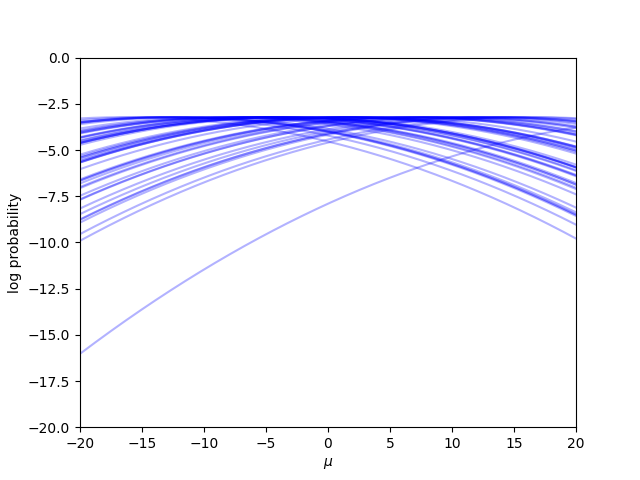
\includegraphics[width=\textwidth]{figs/background/logprob_var_10.png}
        \caption[]{$log(\vec{\theta}_a |\ \vec{y})$}
    \end{subfigure}
    \begin{subfigure}{0.475\textwidth}
        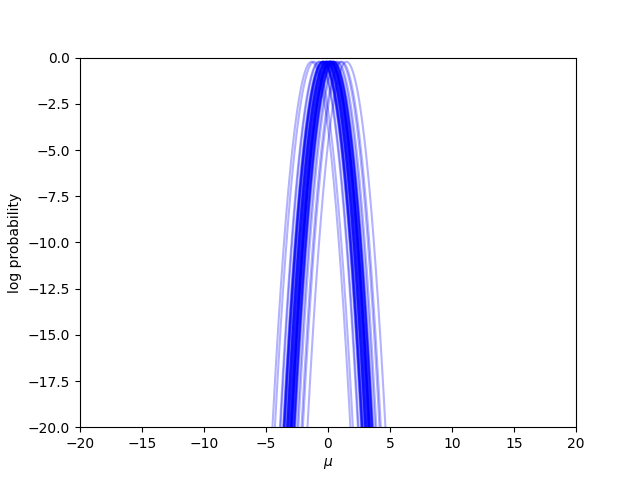
\includegraphics[width=\textwidth]{figs/background/logprob_var_0.5.png}
        \caption[]{$log(\vec{\theta}_b\ |\ \vec{y})$}
    \end{subfigure}
    \caption[Log-likelihood's of observations given a Gaussian distribution]{}
    \label{fig:loglikelihoods}
\end{figure}
\noindent Intuitively from these plots its clear that the low variance case a enables a more accurate estimation of $\mu$ due to the steeper slopes of the log-likelihood function. We obtain these slopes by taking derivative with respect to a model parameter ($\mu$ in this case) of the log-likelihood $\frac{\partial}{\partial\mu} log(\vec{\theta}\ |\ y),\;y\in\vec{y}$ this is known as the score function by convention, we will denote it as $\gls{score}$, note that for more complex functions we assume this derivative exists. For the sake of completeness we show plots of $\mathcal{S}_a$, $\mathcal{S}_b$ for our $\vec{y}$ observations from a and b respectively in \cref{fig:scorefunctions} and the distribution each score function $\mathbb{D}(\mathcal{S})$ when evaluated at the true parameter value $\mu' = 5$ in \cref{fig:scorefunctiondist}.
\begin{figure}
    \centering
    \begin{subfigure}{0.475\textwidth}
        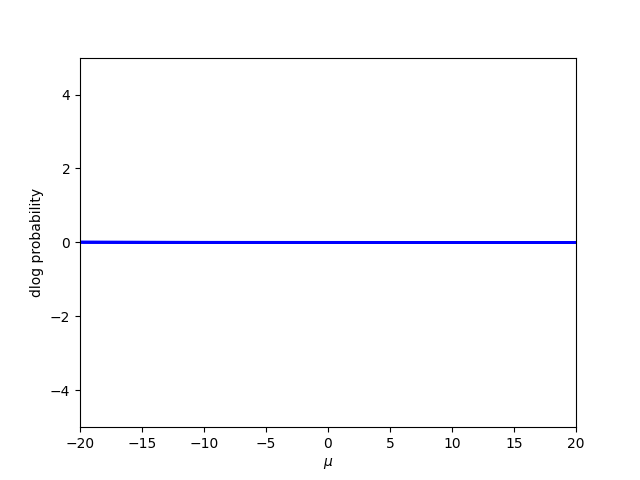
\includegraphics[width=\textwidth]{figs/background/deriv_var_10.png}
        \caption[]{$\frac{\partial}{\partial\mu} log(\vec{\theta}_a |\ \vec{y})$}
    \end{subfigure}
    \begin{subfigure}{0.475\textwidth}
        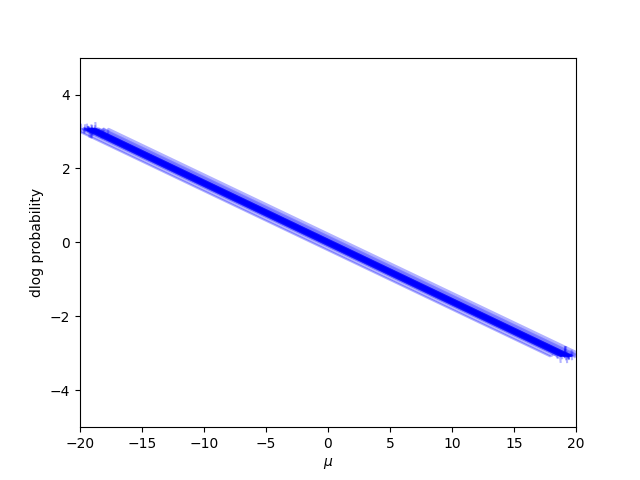
\includegraphics[width=\textwidth]{figs/background/deriv_var_0.5.png}
        \caption[]{$\frac{\partial}{\partial\mu} log(\vec{\theta}_a |\ \vec{y})$}
    \end{subfigure}
    \caption[Score functions of the log-likelihood of observations over $-20<x<20$]{}
    \label{fig:scorefunctions}
\end{figure}
\begin{figure}
    \centering
    \begin{subfigure}{0.475\textwidth}
        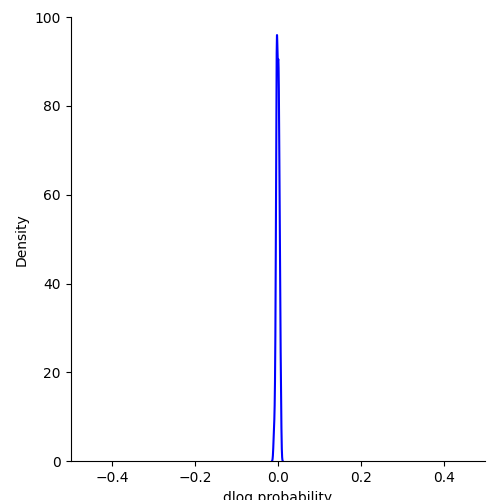
\includegraphics[width=\textwidth]{figs/background/deriv_dist_10.png}
        \caption[]{$\mathbb{D}\left(\frac{\partial}{\partial\mu} log(\vec{\theta}_a |\ \vec{y})\right), \mu'$}
    \end{subfigure}
    \begin{subfigure}{0.475\textwidth}
        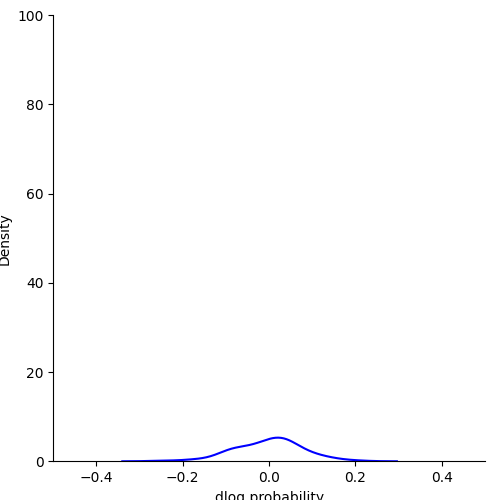
\includegraphics[width=\textwidth]{figs/background/deriv_dist_0.5.png}
        \caption[]{$\mathbb{D}\left(\frac{\partial}{\partial\mu} log(\vec{\theta}_a |\ \vec{y})\right), \mu'$}
    \end{subfigure}
    \caption[Distribution of the score functions when evaluated at $x=\mu'$ ]{}
    \label{fig:scorefunctiondist}
\end{figure}
The Fisher information is beautifully given by the variance of the distribution of the score functions at the true parameter value $\VAR[\mathbb{D}(\mathcal{S}_a)], \mu'$. Calculating $I(\theta)$ from $\vec{y}$ we obtain $I(\theta_a)= 1.77\text{e}-5$ and $I(\theta_b)=5.37\text{e}-3$ confirming initial observations that the low variance case of b provides more information. Note as Fisher information is often used in cases where $\mu'$ is unknown, the secondary and more common method of calculation is to instead take the derivative of the score functions (second derivative of the log-likelihood), the fisher information in then given by \cref{eq:Fisherinfo}. As in a normal distribution the 2nd derivative of the log-likelihood is always a single value we omit plots of the second derivative and it's distribution when evaluated at $\mu'$ for brevity.
\begin{equation}\label{eq:Fisherinfo}
    I(\theta) = -\EX_{\vec{\theta}} \left[
    \frac{\partial^2}{\partial^2\mu} log(y\ |\ \vec{\theta})\right]
\end{equation}
Now considering the multidimensional case of a complex system containing $X=\{x_1,x_2,\ldots,x_n\}$ random variables, each governed by a respective parameter in $\vec{\theta}=\{\theta_1,\theta_2,\ldots,\theta_n\}^T$. Let the value of a single element $x\in X$ in the system have the PDF $f(x\ |\ \theta_x) = y$, with a log-likelihood of $f_{x|\theta_x}(\vec{y}_x)$ where $\theta_x\in \vec{\theta}$ and $y_x$ is the set of observations we make of $x$. We make an additional assumption that that the score function $\forall x\in X,\; \gls{score}:=\frac{\partial}{\partial\mu} f_{x|\theta_x}(y_x)$ is finite (\ie $|X| = n < \infty$). The Fisher information matrix (FIM) \gls{fi} is then the row-major $n\times n$ matrix:
\begin{equation*}
    I(\vec{\theta}) = [I_{ij}(\vec{\theta})^{n}_{i,j=1}]
\end{equation*}
Where the jth element of the ith row is given by:
\begin{equation*}
    I_{ij}(\vec{\theta})= \EX_{\vec{\theta}} \left[
    \frac{\partial}{\partial \theta_i} log f_{x|\vec{\theta}}(y) \cdot
    \frac{\partial}{\partial \theta_j} log f_{x|\vec{\theta}}(y) \right]
\end{equation*}
\noindent This can be simplified by taking the second deviate in a similar fashion to \cref{eq:Fisherinfo} giving:
\begin{equation}\label{eq:FIM}
    I_{ij}(\vec{\theta})= -\EX_{\vec{\theta}}\left[
    \frac{\partial^2}{\partial \theta_i \partial \theta_j} log f_{x|\vec{\theta}}(y)\right]
\end{equation}
This matrix concisely represents the co-variance of all MLEs, with the co-variance of the $i$th and $j$th parameters estimator given by $\gls{fi}_{ij}$ and the variance of the estimator of parameter $n\equiv\gls{fi}_{nn}$.

\subsection{The Cramér–Rao Bound}
\label{ssec:Bcrb}

Given $I(\theta)$ the Cramér–Rao Bound (CRB) gives a lower bound on the accuracy with which we can estimate each $\theta\in\hat\theta$. From \cref{ssec:Bmle} we know that $\VAR(\gls{mle})$ dictates our confidence that the MLE reflects the true value of the parameter, it follows that the CRB is simply a bound on $\VAR(\gls{mle})$, we provide a proof from \cite{trees_detection_2013} under the assumption that the MLE is unbiased.
\begin{lemma}\label{lem:dx1}
Given an unbiased estimator $\int f\ dx=1$ 
\end{lemma}
\begin{align*}
    0 &= \EX[\hat\theta - \theta\ |\ \theta]\\
    &= \int (\hat\theta - \theta) f(x\ |\ \theta)dx\\
    &= \frac{\partial}{\partial\theta}\int \hat\theta - \theta) f(x\ |\ \theta)dx\\
    &= \int \hat\theta - \theta) f(x\ |\ \theta)\frac{\partial}{\partial\theta}dx-\int f\ dx\\
    &\therefore \int f\ dx = 1
\end{align*}
Using lemma 3.4.1 and the intuitive equality $\frac{\partial f}{\partial\theta} = f\frac{\partial log f}{\partial\theta}$ it follows:
\begin{equation}\label{eq:crbderivation}
\begin{aligned}
    \int(\hat\theta-\theta)\ \frac{\partial logf}{\partial\theta}dx = 1\\
    \int((\hat\theta-\theta)\sqrt{f})\cdot\left(\sqrt{f}\ \frac{\partial logf}{\partial\theta}\right) dx = 1\\
    \left[\int(\hat\theta -\theta)^2 f\ dx\right]\cdot
    \left[\int\left(\frac{\partial logf}{\partial\theta}\right)^2 f\ dx\right] \geq
    \left(\int((\hat\theta-\theta)\sqrt{f})\cdot
    \left(\sqrt{f}\ \frac{\partial logf}{\partial\theta}\right) dx\right)^2 = 1\\
\end{aligned}
\end{equation}
From rearranging the equality in \cref{eq:crbderivation} we have $\VAR(\hat\theta) \geq 1/I(\theta)$.\par
For the multi-parameter case of a FIM, instead of $\VAR(\widehat{\mathcal{L}})$, the CRB is w.r.t. the co-variance matrix $cov_\theta(\hat\theta)$ where $\hat\theta$ is the vector of MLE's for each  $\theta\in\vec{\theta}$ and $\vec{\theta}=\{\theta_1,\theta_2,\ldots,\theta_n\}^T$. The CRB is then given by the inequality $cov_\theta(\hat\theta)\geq \gls{fi}^{-1}$, we note that in cases where $n>>1$, $\gls{fi}^{-1}$ is infeasible to compute, in these cases a looser bound can be given using only the diagonal elements on the inverse matrix by $\sum_{i=1}^n 1/I(\hat\theta)_{ii}^{-1}$ as:
\begin{align*}
    \VAR_{\vec{\theta}}(\hat\theta) &= [cov_{\vec{\theta}}(\hat\theta)]_{ii}\\
    &\geq [I(\vec{\theta})]^{-1}_{ii}\\
    &\geq [I(\vec{\theta})_{ii}]^{-1}
\end{align*}

\section{Optimization Techniques}
\label{sec:Boptimization}
The accuracy of tomographic analysis is intuitively bound by the information acquired from measurements and how we process that information. In this section we introduce techniques for maximising the information we are able to gain from our probing by decomposing the measurement process into two stages: selection of paths to probe and allocation of probes over these paths. In \cref{ssec:Bparsppselection} we address the first of these stages, explaining the desire for a minimal number of paths and presenting Zheng's algorithm for selecting this minimal set of paths. Next in \cref{ssec:Boptimumdesigns} we cover relevant core concepts in the field of optimum experimental design with the intent of using these in the context of probe allocation to paths in \cref{ssec:Mpallocation}.

\subsection{Parsimonious Probe Path Selection}
\label{ssec:Bparsppselection}

With a scope limited to tree network topologies \cite{lawrence_network_2006} focused on deriving an algorithm for an optimal selection of a set of probe paths $P^*$ for network tomography. We define an optimal selection of probe paths as the minimal set of probe paths that allow for complete node identifiability. Such a minimal set is desirable as when probing we allocate probe packets over each path $p\in P^*$, reducing the amount of information we gain about a path proportionally to the number of probe allocated to it. To ensure our inference is robust and has a maximal CRB (discussed in \cref{ssec:Bcrb}) we aim to gain as much data over the measurement interval as possible and adopt a parsimonious approach where we aim to select a $P^*$ s.t. \cref{eq:minpp} holds where $P$ is the set of all possible probe paths.
\begin{equation}
\label{eq:minpp}
    I(P^*) = I(P)
\end{equation}
\par
The problem of rigorously minimizing $P^*$ has been shown to be NP-hard by \cite{zheng_minimizing_2013}. However polynomial time solutions using a heuristic based approach for an approximation of a minimal $P*$ in general topologies have been derived previous and three notable methods have been developed: Zheng's algorithm (\cite{zheng_minimizing_2013}), Evolutionary Sampling algorithm (\cite{rahali_unicast_2019}), and Greedy-Min-Cost-Rank (\cite{tootaghaj_parsimonious_2018}). As the Evolutionary Sampling algorithm (ESA) was developed under the assumption of central monitors where all probe path metrics are compiled contrasting our assumption of observability of all monitors we do not consider ESA.\par
\captionsetup{justification=centering}
\begin{figure}[H]
    \centering
    \tikzsetnextfilename{bipartitegraph}
    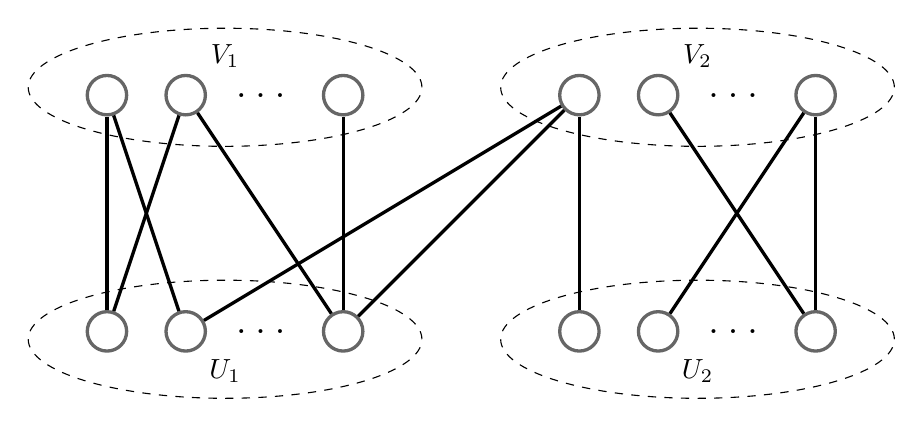
\begin{tikzpicture}[
        node/.style={circle, draw=black!60, very thick, minimum size=5mm},
        group/.style={circle, draw=black!60, very thick, minimum size=5mm},]
        
        % Nodes
        \node[node] (v10) at (-6.5,1.5) {};
        \node[node] (v11) at (-5.5,1.5) {};
        \node at (-4.5,1.5) {{\LARGE\ldots}};
        \node[node] (v12) at (-3.5,1.5) {};
        
        \node[node] (u10) at (-6.5,-1.5) {};
        \node[node] (u11) at (-5.5,-1.5) {};
        \node at (-4.5,-1.5) {{\LARGE\ldots}};
        \node[node] (u12) at (-3.5,-1.5) {};
        
        \node[node] (v20) at (-0.5,1.5) {};
        \node[node] (v21) at (0.5,1.5) {};
        \node at (1.5,1.5) {{\LARGE\ldots}};
        \node[node] (v22) at (2.5,1.5) {};
        
        \node[node] (u20) at (-0.5,-1.5) {};
        \node[node] (u21) at (0.5,-1.5) {};
        \node at (1.5,-1.5) {{\LARGE\ldots}};
        \node[node] (u22) at (2.5,-1.5) {};
        
        % Groups
        \draw[dashed] (-5,1.6) ellipse (2.5cm and 0.75cm);
        \draw[dashed] (-5,-1.6) ellipse (2.5cm and 0.75cm);
        \draw[dashed] (1,1.6) ellipse (2.5cm and 0.75cm);
        \draw[dashed] (1,-1.6) ellipse (2.5cm and 0.75cm);
        
        % Edges
        \draw[very thick] (v10) -- (u10);
        \draw[very thick] (v10) -- (u11);
        \draw[very thick] (v11) -- (u12);
        \draw[very thick] (v11) -- (u10);
        \draw[very thick] (v12) -- (u12);
        \draw[very thick] (v20) -- (u11);
        \draw[very thick] (v20) -- (u12);
        \draw[very thick] (v21) -- (u22);
        \draw[very thick] (v20) -- (u20);
        \draw[very thick] (v22) -- (u21);
        \draw[very thick] (v22) -- (u22);
        
        % Labels
        \node at (-5,2) {$V_1$};
        \node at (-5,-2) {$U_1$};
        \node at (1,2) {$V_2$};
        \node at (1,-2) {$U_2$};
    \end{tikzpicture}
    \caption[Extended bipartite model of the network for probe path selection.]{Extended bipartite model of the network for probe path selection.}
    \label{fig:ebgm}
\end{figure}
Both Greedy-Min-Cost-Rank (GMCR) and Zheng's algorithm minimize the probing cost in a context analogous to ours, however the key difference is in definition of probing cost. In Zheng's algorithm the probing cost is defined as $|P^*|$ whereas in GMCR it is the total number of 'hops' or nodes in all paths $\forall p_i\in P^*,\ \sum |p_i|$. Although developed for the purpose of link tomography \cite{zheng_minimizing_2013} note it's applicability to node tomography we therefore adopt Zheng's algorithm \cref{alg:zhengs} for it's alignment with our goal of minimizing $|P^*|$. The core idea behind Zheng's algorithm is quantifying the contribution of a probe path to node identifiability and then adopting a greedy selection approach until all nodes are identifiable. The criteria used for the greedy is based on a novel extended bipartite graph model (EBGM) shown in \cref{fig:ebgm}.\par
This graph model groups network nodes into $V_1$ or $V_2$ based on if the node is identifiable or not. The group $U_1$ contains sets of probe paths that enable identification of a node in $V_1$, with an edge connecting a node in $V_1$ and $U_2$ if the set of paths in $U_2$ enables identification of $V_1$. Similarly $U_2$ contains probe paths which traverse a node in $V_2$, with an edge connecting a node in $V_2$ and $U_2$ if the path traverses that node.
\begin{algorithm}
    \KwData{The linear system $L$ and parameter $\alpha$}
    \KwResult{Minimal set of probe paths $P^*$}
    
    \For{each node}{
        Calculate $\alpha$ solutions using $A$ and $L$\;
    }
    Construct the extended bipartite graph $G'=(U,V,E)$ with the selected solutions\;
    $P^* \gets \varnothing$ \;
    $C \gets \varnothing$ \;
    \While{$\exists\ n \in V_1,\ n\not\in C$}{
        $u_{selected} \gets u_x\in U_1\ \text{with max}\left(\frac{|newV2|}{|newpaths|}\right)$ where: $newV2 = v_i\in V_2 - C,\ \{v_i, u_x\}\in E$ and $newpaths = p_i\in u_x,\ p_i \not\in P_s$\;
        $C \gets C + u_{selected}$\;
        $C \gets v_i \in V_1\cup V_2,\ \{v_i, u_{selected}\}\in E$\;
        \For {$p_i \in u_{selected}, p_i \not\in P^*$}{
            $P^* \gets P^* + p_i$\;
        }
    }
    \While{$\exists\ n \in V_2,\ n\not\in C$}{
        $u_{selected} \gets u_x\in U_1\cup U_2\ \text{with max}\left(\frac{|newV1|}{|newpaths|}\right)$ where: $newV1 = v_i\in V_1 - C,\ \{v_i, u_x\}\in E$ and $newpaths = p_i\in u_x,\ p_i \not\in P_s$\;
        $C \gets C + u_{selected}$\;
        $C \gets v_i \in V_1\cup V_2,\ \{v_i, u_{selected}\}\in E$\;
        \For {$p_i \in u_{selected}, p_i \not\in P^*$}{
            $P^* \gets P^* + p_i$\;
        }
    }
    Remove all replaceable probing paths from set $P^*$ using $L$\;
    \caption{Zheng's minimal probe path selection algorithm}
    \label{alg:zhengs}
\end{algorithm}

\subsection{Optimum Experiment Design}
\label{ssec:Boptimumdesigns}

Optimum experiment design (OED) is board field of study focusing on statistical methods to ensure an experiment yields the most robust and accurate results possible. Initially shepherded by \cite{smith_standard_1918}, of particular pertinence to tomography is OEDs applicability to parameter estimation in inverse problems. Work around OED for parameter estimation, as noted in \cref{cha:litreview}, primarily focuses on minimising the number of trials or "experimental cost" for accurately estimating a system's underlying statistical models, this lens can be inverted to instead maximise the accuracy of this estimation from a fixed number of trials.\par
At a high level, the problem of designing an optimal experiment is typically decomposed into 4 primary sub-problems: specification of a model, identification of the design region, specification of a design criterion, and specification of errors. If the formulated design differs significantly from popular existing approaches in literature a comparison should be drawn to validate key differences or identify missteps in problem specification. Irrelevant of its formulation, the experiment produces an estimator of the underlying parameters and is evaluated w.r.t the variance of this estimator as, intuitively, the variance of the estimator corresponds to the accuracy of the experiment.\par
Experiments to infer complex model\footnote{A complex model is analogous to the mathematical representation of a multi-parametric system such as a computer network.} parameters (sometimes referred to as screening experiments) can be evaluated using a range of statistical criteria however the two most common are A-optimality and D-optimality. A-optimality minimizes the average variance of all parameter estimates or, as the diagonal elements of the FIM correspond to these variances (\cref{ssec:Bfisherinformation}), the trace of the FIM tr$\left(\gls{fi}\right)$. In contrast D-optimality minimises the confidence region around the estimators, as this confidence region is inversely proportional to the determinant of the FIM (\cite{jones_-optimal_2021}) this is equivalent to maximising $|\gls{fi}|$.\par

\section{Summary}

In this chapter we introduced...  \todo{mention the story in next chapter}